%%%%%%%%%%%%%%%%%%%%%%%%%%%%%%%%%%%%%%%%%
% Document Author: Plinio H. Vargas
% Course: CS-532, Spring 2016 at Old Dominion University
%
% Structured General Purpose Assignment
% LaTeX Template
%
% This template has been downloaded from:
% http://www.latextemplates.com
%
% Original template author:
% Ted Pavlic (http://www.tedpavlic.com)
%
% Note:
% The \lipsum[#] commands throughout this template generate dummy text
% to fill the template out. These commands should all be removed when 
% writing assignment content.
%
%%%%%%%%%%%%%%%%%%%%%%%%%%%%%%%%%%%%%%%%%
%----------------------------------------------------------------------------------------
%	PACKAGES AND OTHER DOCUMENT CONFIGURATIONS
%----------------------------------------------------------------------------------------

\documentclass{article}

\usepackage{fancyhdr} % Required for custom headers
\usepackage{lastpage} % Required to determine the last page for the footer
\usepackage{extramarks} % Required for headers and footers
\usepackage{listings}
\usepackage{graphicx} % Required to insert images
\usepackage{lipsum} % Used for inserting dummy 'Lorem ipsum' text into the template
\usepackage[bookmarks,bookmarksopen,bookmarksdepth=2]{hyperref} % for bookmarks
\usepackage{enumerate}
\usepackage{csquotes} % for quoting things
\usepackage{multirow}
\usepackage{amsmath}
\usepackage{caption}
\usepackage{navigator}%\usepackage{caption}
\usepackage[shortlabels]{enumitem}
\usepackage{enumitem}
\usepackage{lmodern}
\usepackage[utf8]{inputenc}
%\usepackage[table]{xcolor}% http://ctan.org/pkg/xcolo
\usepackage[dvipsnames]{xcolor}
\usepackage{longtable}
\usepackage{textcomp}
\usepackage{url}
\usepackage{import}
\usepackage{float}
\usepackage{dashrule} % for dashline
\usepackage{keystroke}
\usepackage{amssymb}
\usepackage{booktabs}

\lstdefinestyle{numbers}
{ frame=tb,
  language=python,
  aboveskip=3mm,
  belowskip=3mm,
  showstringspaces=false,
  columns=flexible,
  basicstyle={\small\ttfamily},
  numbers=left,
  numberstyle=\tiny\color{gray},
  keywordstyle=\color{blue},
  commentstyle=\color{OliveGreen},
  stringstyle=\color{purple},
  breaklines=true,
  breakatwhitespace=true,
  tabsize=3
}

\lstdefinestyle{nonumbers}
{ frame=shadowbox,
  language=python,
  aboveskip=3mm,
  belowskip=3mm,
  showstringspaces=false,
  columns=flexible,
  basicstyle={\small\ttfamily},
  numbers=none,
  numberstyle=\tiny\color{gray},
  keywordstyle=\color{blue},
  commentstyle=\color{OliveGreen},
  stringstyle=\color{purple},
  breaklines=true,
  breakatwhitespace=true,
  tabsize=3
}

\lstdefinestyle{mybox}
{
	basicstyle={\small\ttfamily},
    numbers=left,
    numberstyle=\tiny\color{gray},
    stepnumber=1,
    numbersep=5pt,
    showspaces=false, % don't show spaces by adding underscores
    showstringspaces=false, % don't underline spaces in strings
    showtabs=false, % don't show tabs with underscores
    frame=shadowbox,
    tabsize=4,
    captionpos=b,
    breaklines=true,
    breakatwhitespace=false,
  	keywordstyle=\color{blue},
	commentstyle=\color{OliveGreen},
  	stringstyle=\color{purple},    
    rulesepcolor=\color{red!20!green!20!blue!20},
    numberbychapter=false,
    stringstyle=\color{purple},
}


\providecommand{\providehyphenmins}[2]{}

% Margins
\topmargin=-0.45in
\evensidemargin=0in
\oddsidemargin=0in
\textwidth=6.5in
\textheight=9.0in
\headsep=0.25in 

\linespread{1.1} % Line spacing
\newcommand*{\medtau}{\mathbin{\scalebox{1.5}{$\tau$}}}% increase size of tau
\newcommand*{\medtaub}{\mathbin{\scalebox{1.5}{$\tau_b$}}}% increase size of tau_b
\newcommand\multibrace[3]{\rdelim\}{#1}{3mm}[\pbox{#2}{#3}]}

% Set up the header and footer
\pagestyle{fancy}
\lhead{\hmwkAuthorName} % Top left header
\chead{\hmwkShortClass\ (\hmwkClassInstructor\ \hmwkClassTime): \hmwkShortTitle} % Top center header
%\rhead{\firstxmark} % Top right header
\rhead{} % Top right header
\lfoot{\lastxmark} % Bottom left footer
\cfoot{} % Bottom center footer
\rfoot{Page\ \thepage\ of\ \pageref{LastPage}} % Bottom right footer
\renewcommand\headrulewidth{0.4pt} % Size of the header rule
\renewcommand\footrulewidth{0.4pt} % Size of the footer rule

\setlength\parindent{0pt} % Removes all indentation from paragraphs

%----------------------------------------------------------------------------------------
%	DOCUMENT STRUCTURE COMMANDS
%	Skip this unless you know what you're doing
%----------------------------------------------------------------------------------------

% Header and footer for when a page split occurs within a problem environment
\newcommand{\enterProblemHeader}[1]{
\nobreak\extramarks{#1}{#1 continued on next page\ldots}\nobreak
\nobreak\extramarks{#1 (continued)}{#1 continued on next page\ldots}\nobreak
}

% Header and footer for when a page split occurs between problem environments
\newcommand{\exitProblemHeader}[1]{
\nobreak\extramarks{#1 (continued)}{#1 continued on next page\ldots}\nobreak
\nobreak\extramarks{#1}{}\nobreak
}

\newcounter{sub}[section]
\newenvironment{sub}[1][]{\stepcounter{sub}\thesub #1}{ }

\setcounter{secnumdepth}{4} % Removes default section numbers
\newcounter{homeworkProblemCounter} % Creates a counter to keep track of the number of problems
\newcommand{\sectionNumber}{\arabic{homeworkProblemCounter}.\sub }


\newcommand{\homeworkProblemName}{}
\newenvironment{homeworkProblem}[1][Problem \arabic{homeworkProblemCounter}]{ % Makes a new environment called homeworkProblem which takes 1 argument (custom name) but the default is "Problem #"
\stepcounter{homeworkProblemCounter} % Increase counter for number of problems
\setcounter{sub}{0}
\renewcommand{\homeworkProblemName}{#1} % Assign \homeworkProblemName the name of the problem
\
\section{\homeworkProblemName} % Make a section in the document with the custom problem count
\enterProblemHeader{\homeworkProblemName} % Header and footer within the environment
}{
\exitProblemHeader{\homeworkProblemName} % Header and footer after the environment
}

\newcommand{\problemAnswer}[1]{ % Defines the problem answer command with the content as the only argument
\noindent\framebox[\columnwidth][c]{\begin{minipage}{0.98\columnwidth}#1\end{minipage}} % Makes the box around the problem answer and puts the content inside
}

\newcommand{\homeworkSectionName}{}
\newenvironment{homeworkSection}[1]{ % New environment for sections within homework problems, takes 1 argument - the name of the section
\renewcommand{\homeworkSectionName}{#1} % Assign \homeworkSectionName to the name of the section from the environment argument
\subsection{\homeworkSectionName} % Make a subsection with the custom name of the subsection
\enterProblemHeader{\homeworkProblemName\ [\homeworkSectionName]} % Header and footer within the environment
}{
\enterProblemHeader{\homeworkProblemName} % Header and footer after the environment
}
   
%----------------------------------------------------------------------------------------
%	NAME AND CLASS SECTION
%----------------------------------------------------------------------------------------

\newcommand{\hmwkTitle}{\\Assignment\ \#2: \\Ex 4.1, 4.2, 4.3, 4.8 \& 5.10} % Assignment title
\newcommand{\hmwkShortTitle}{Assignment 2} % Assignment title
\newcommand{\hmwkDueDate}{Thursday,\ October 12,\ 2016} % Due date
\newcommand{\hmwkClass}{CS-734/834 Introduction to Information Retrieval} % Course/class
\newcommand{\hmwkShortClass}{CS-734/834 Intro to IR} % Course/class
\newcommand{\hmwkClassTime}{- Fall 2016} % Class/lecture time
\newcommand{\hmwkClassInstructor}{Dr.  Michael L. Nelson} % Teacher/lecturer
\newcommand{\hmwkAuthorName}{Plinio Vargas} % Your name
\newcommand{\hmwkAuthorEmail}{pvargas@cs.odu.edu} % Your name
%------------------------------------------------------------
% Algorithm declaration
%------------------------------------------------------------
\lstnewenvironment{algorithm}[1][] %defines the algorithm listing environment
{   
    %\refstepcounter{nalg} %increments algorithm number
    \captionsetup{labelsep=colon} %defines the caption setup for: it ises label format as the declared caption label above and makes label and caption text to be separated by a ':'
    \lstset{ %this is the stype
        frame=tB,
        numbers=left, 
        mathescape=true,
        numberstyle=\tiny,
        basicstyle={\small\ttfamily}, 
        keywordstyle=\color{blue}\bfseries\em,
        keywords={,input, output, return, 
                   datatype, function, in, 
                   if, else, for, foreach, 
                   while, write, begin, end, 
        } %add the keywords you want, or load a language as Rubens explains in his comment above.
        numbers=left,
        xleftmargin=.04\textwidth,
        #1 % this is to add specific settings to an usage of this environment (for instnce, the caption and referable label)
    }
}
{}
%----------------------------------------------------------------------------------------
%	TITLE PAGE
%----------------------------------------------------------------------------------------

\title{
\vspace{2in}
\textmd{\textbf{\hmwkClass:\ \hmwkTitle}}\\
\normalsize\vspace{0.1in}\small{Due\ on\ \hmwkDueDate}\\
\vspace{0.1in}\large{\textit{\hmwkClassInstructor\ }}
\vspace{3in}
}

\author{\textbf{\hmwkAuthorName} \\ \hmwkAuthorEmail}
\date{} % Insert date here if you want it to appear below your name

%----------------------------------------------------------------------------------------
%	EMBEDDED FILE
%----------------------------------------------------------------------------------------
%\embeddedfile{KarateClub}{../KarateClub.py}
%\embeddedfile{DrawOriginalClub}{../DrawOriginalClub.py}
%----------------------------------------------------------------------------------------
%	START OF DOCUMENT
%----------------------------------------------------------------------------------------
\begin{document}

\clearpage\maketitle
\thispagestyle{empty}

%----------------------------------------------------------------------------------------
%	TABLE OF CONTENTS
%----------------------------------------------------------------------------------------

%\setcounter{tocdepth}{1} % Uncomment this line if you don't want subsections listed in the ToC

\newpage
\clearpage\tableofcontents
\listoffigures
\lstlistoflistings
\listoftables

\thispagestyle{empty}
\newpage
\setcounter{page}{1}

%Exercices on pages: 35,52,
%----------------------------------------------------------------------------------------
%	Problem 1
%----------------------------------------------------------------------------------------
\begin{homeworkProblem}[Exercise 4.1]% Custom section title
\vspace*{10pt} % Question
Plot rank-frequency curves (using a log-log graph) for words and bigrams in
the Wikipedia collection available through the book website (http://www.searchengines-
book.com). Plot a curve for the combination of the two. What are the best
values for the parameter c for each curve?\\

\subsection{Approach}
The collection available in the book's website was downloaded from \url{http://www.search-engines-book.com/collections/}. There are various collections within the site.  Experiments were performed initially with the small collection (\textbf{Wiki small}) which contains 6,043 documents. Although plotting a \textbf{Zipf curve} will work better in large collections, the small collection helped in the testing and  the debugging of our script.\\

The script \textbf{zipf\_curve.py} was developed to tokenize the collection. It also produced the data (\textit{zipf\_law*.txt}) required to plot the curves. The ``R'' script \textbf{zipf\_law.R} was developed to plot and find the best \textit{c} for each curve.\\

\subsubsection{Running Zipf\_curve.py}

\begin{figure}[h]\caption{Running zipt\_curve.py from Command Line} \label{fig:run-zipf-curve}
	\center
	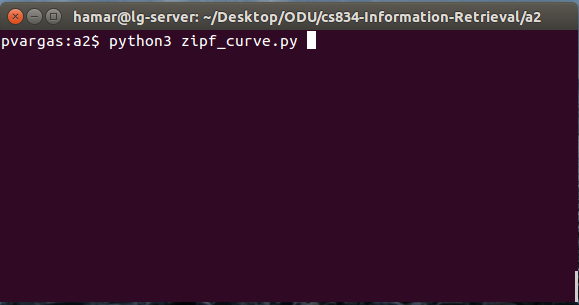
\includegraphics[scale=0.5]{images/run-zipf-curve.png}
\end{figure} 
%--------------
%  P1 tokenization
%--------------
\subsubsection{Collection Tokenization}
The collection was installed in folder \textbf{./en} (line 27 Listing \ref{listing:zipf_curve}). \textbf{zipf\_curve.py}  recursively read all documents until reaching the bottom of the tree. Since the documents are in a \textbf{HTML} format, the library \textbf{BeautifuSoup} was utilized to extract the words from the documents. Then, it followed a similar approach proposed in the textbook \cite{CroftMetzlerStrohman} by:
\begin{enumerate}
	\item Transforming all words to \textbf{lowercase}. Line 74.
	\item Replacing with blanks some special characters that were not bringing additional meaning to a word, such as ?, \&, *, etc. Line 67. This step required running the program various times and checking the index to see which unigrams were created that did not requir to be tokenized.
\end{enumerate}

%--------------
%  zipf_curve.py
%--------------
\lstinputlisting[language=Python,
                 style=mybox, 
                 captionpos=t,
                 caption={zipf\_curve.py},
				 linerange={16-105},
				 firstnumber=16,                  
                 label=listing:zipf_curve,
                 ]
{../zipf_curve.py}

%--------------
%  P1 tokenization
%--------------
\subsubsection{Data Collection}
Per requirement, the collection MUST be tokenized using \textit{unigram} and \textit{bigram} tokens. \textbf{zipf\_curve.py} made two iterations: 
\begin{enumerate}
	\item Find the \textit{unigrams} and their frequency within a document. Lines 72-84.
	\item Once the token discrimination had been performed in the previous step, the side by side word pairing was performed in memory to obtain the \textit{bigrams}. Lines 90-95.
\end{enumerate}

The word frequency is added to its collection every time a word is extracted. The word frequency is added to a dictionary structure that contains all the words and their frequency in the collection. Lines 80 and 94.

\subsection{Solution}
\begin{figure}[h]\caption{Result from \textbf{zipt\_curve.py} Small Collection} \label{fig:run-zipf-res}
	\center
	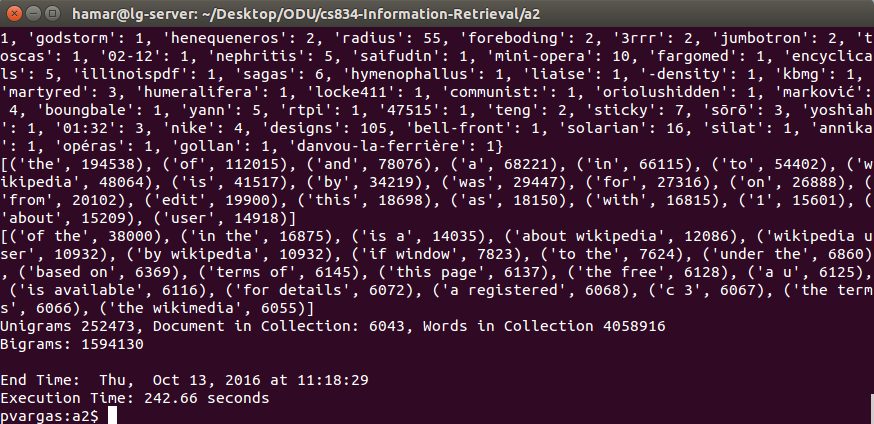
\includegraphics[scale=0.4]{images/zipf-curve-result-s.png}
\end{figure} 

\begin{figure}[h]\caption{Result from \textbf{zipt\_curve.py} Large Collection} \label{fig:run-zipf-res-l}
	\center
	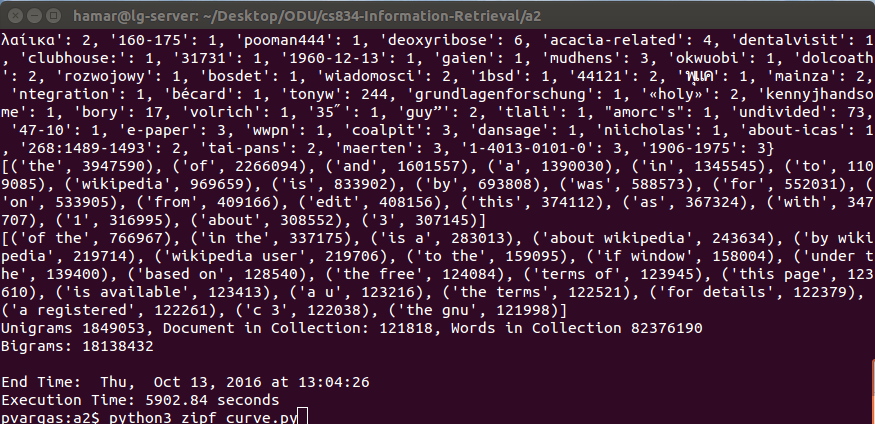
\includegraphics[scale=0.4]{images/zipf-curve-result-l.png}
\end{figure} 
\begin{table}[h] \label{tab:wiki-collection}
\begin{center}
\caption{Wikipedia Collection}
\begin{tabular}{lrr}
\toprule
& \multicolumn{1}{c}{Small} & \multicolumn{1}{c}{Large}\\
\midrule
Total Documents & 6,043 & 121,818\\
Total Word Occurrences & 4,058,916 & 82,376,190\\
Number of Unigrams & 252,473 & 1,849,053\\
Number of Bigrams & 1,594,130 & 18,138,432\\
\bottomrule
\end{tabular}
\end{center}
\end{table}

\newpage
\begin{figure}[h]\caption{Unigram Zipf-Curve} \label{fig:unigram-zipf-small}
	\center
	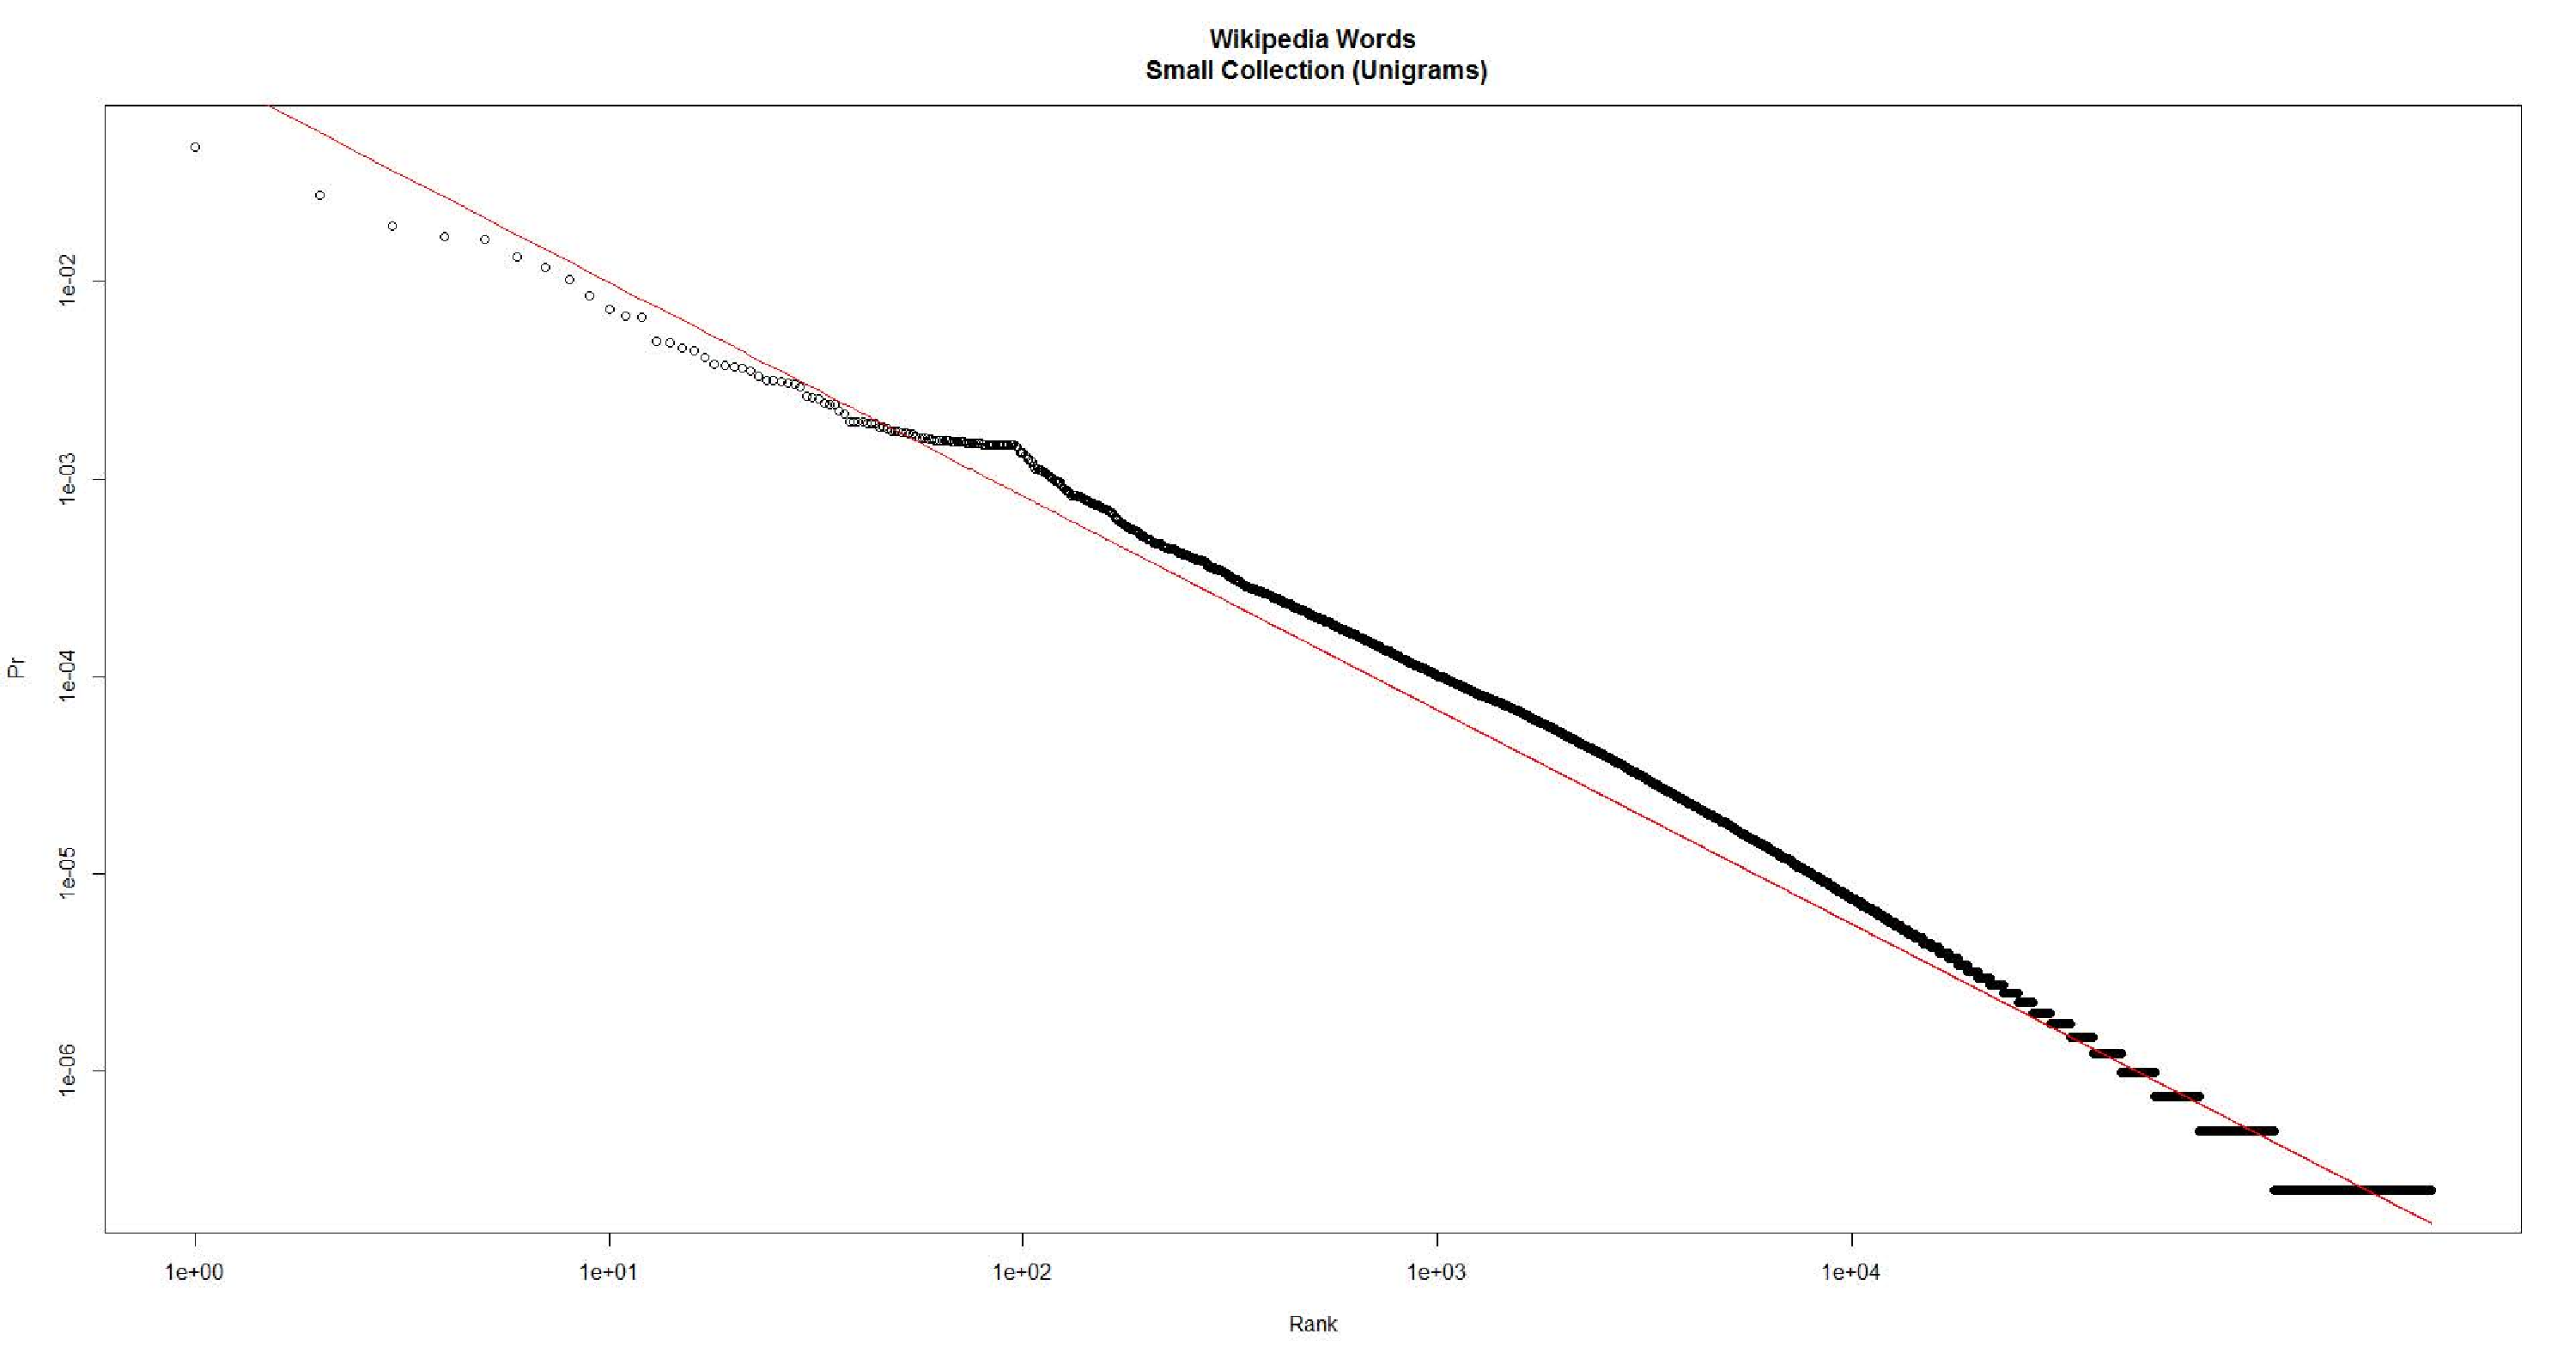
\includegraphics[scale=0.3]{images/zipf_cuve_s_unigram.pdf}
\end{figure} 

\begin{verbatim}
Maximum likelihood estimation

Call:
mle(minuslogl = ll, start = list(s = 1.08007))

Coefficients:
  Estimate   Std. Error
s 1.010182 0.0001326132

-2 log L: 67871958 
> exp(lzipf(s.sq,max_x))[1]
[1] 0.1204752
\end{verbatim}

Estimation for C in Wikipedia unigram small collection is \textbf{0.1204752}

\newpage
\begin{figure}[h]\caption{Bigram Zipf-Curve} \label{fig:bigram-zipf-small}
	\center
	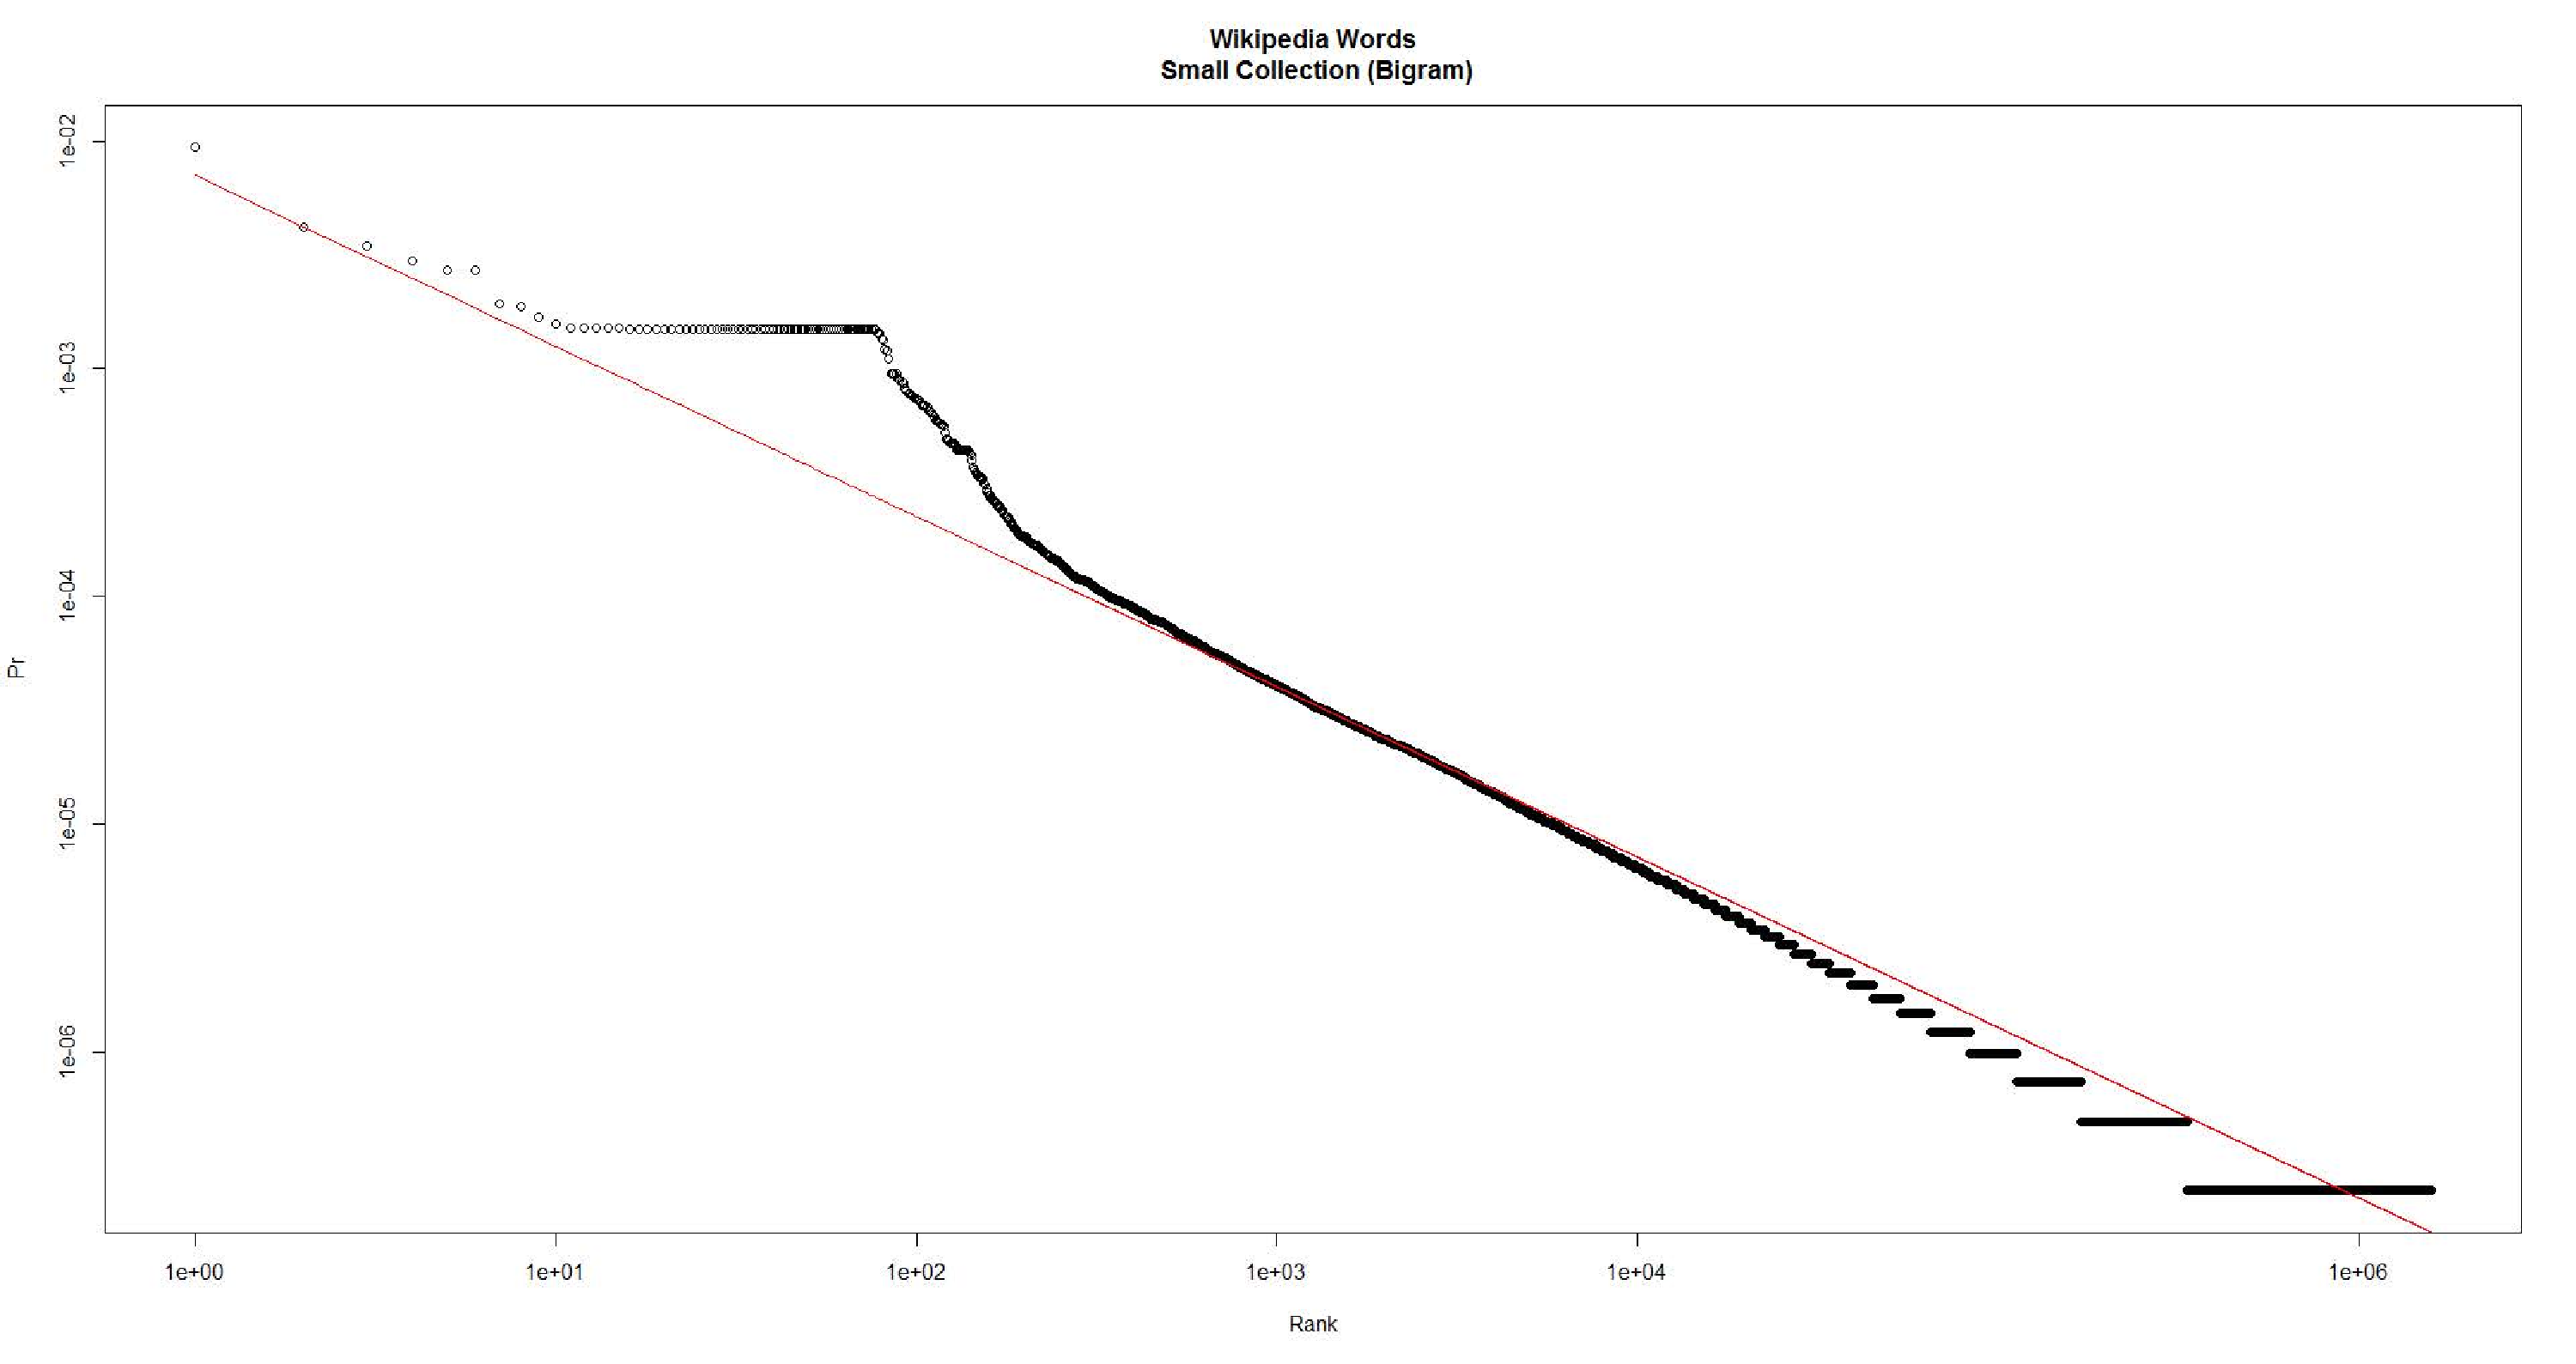
\includegraphics[scale=0.3]{images/zipf_cuve_s_bigram.pdf}
\end{figure} 

\begin{verbatim}
Maximum likelihood estimation

Call:
mle(minuslogl = ll, start = list(s = 1))

Coefficients:
   Estimate  Std. Error
s 0.8194184 0.000136322

-2 log L: 99517651 
> exp(lzipf(s.sq,max_x))[1]
[1] 0.1123482
\end{verbatim}

Estimation for C in Wikipedia bigram small collection is \textbf{0.1123482}

\newpage
\subsubsection{Combined Curve}
We can find the value of $C$ for the combined curves in Figure \ref{fig:combine-zipf-small} by getting the coefficient for the best fitted line in the log graph.  Calculation in \textbf{R} provides: 

\begin{figure}[h]\caption{Combine Zipf-Curve} \label{fig:combine-zipf-small}
	\center
	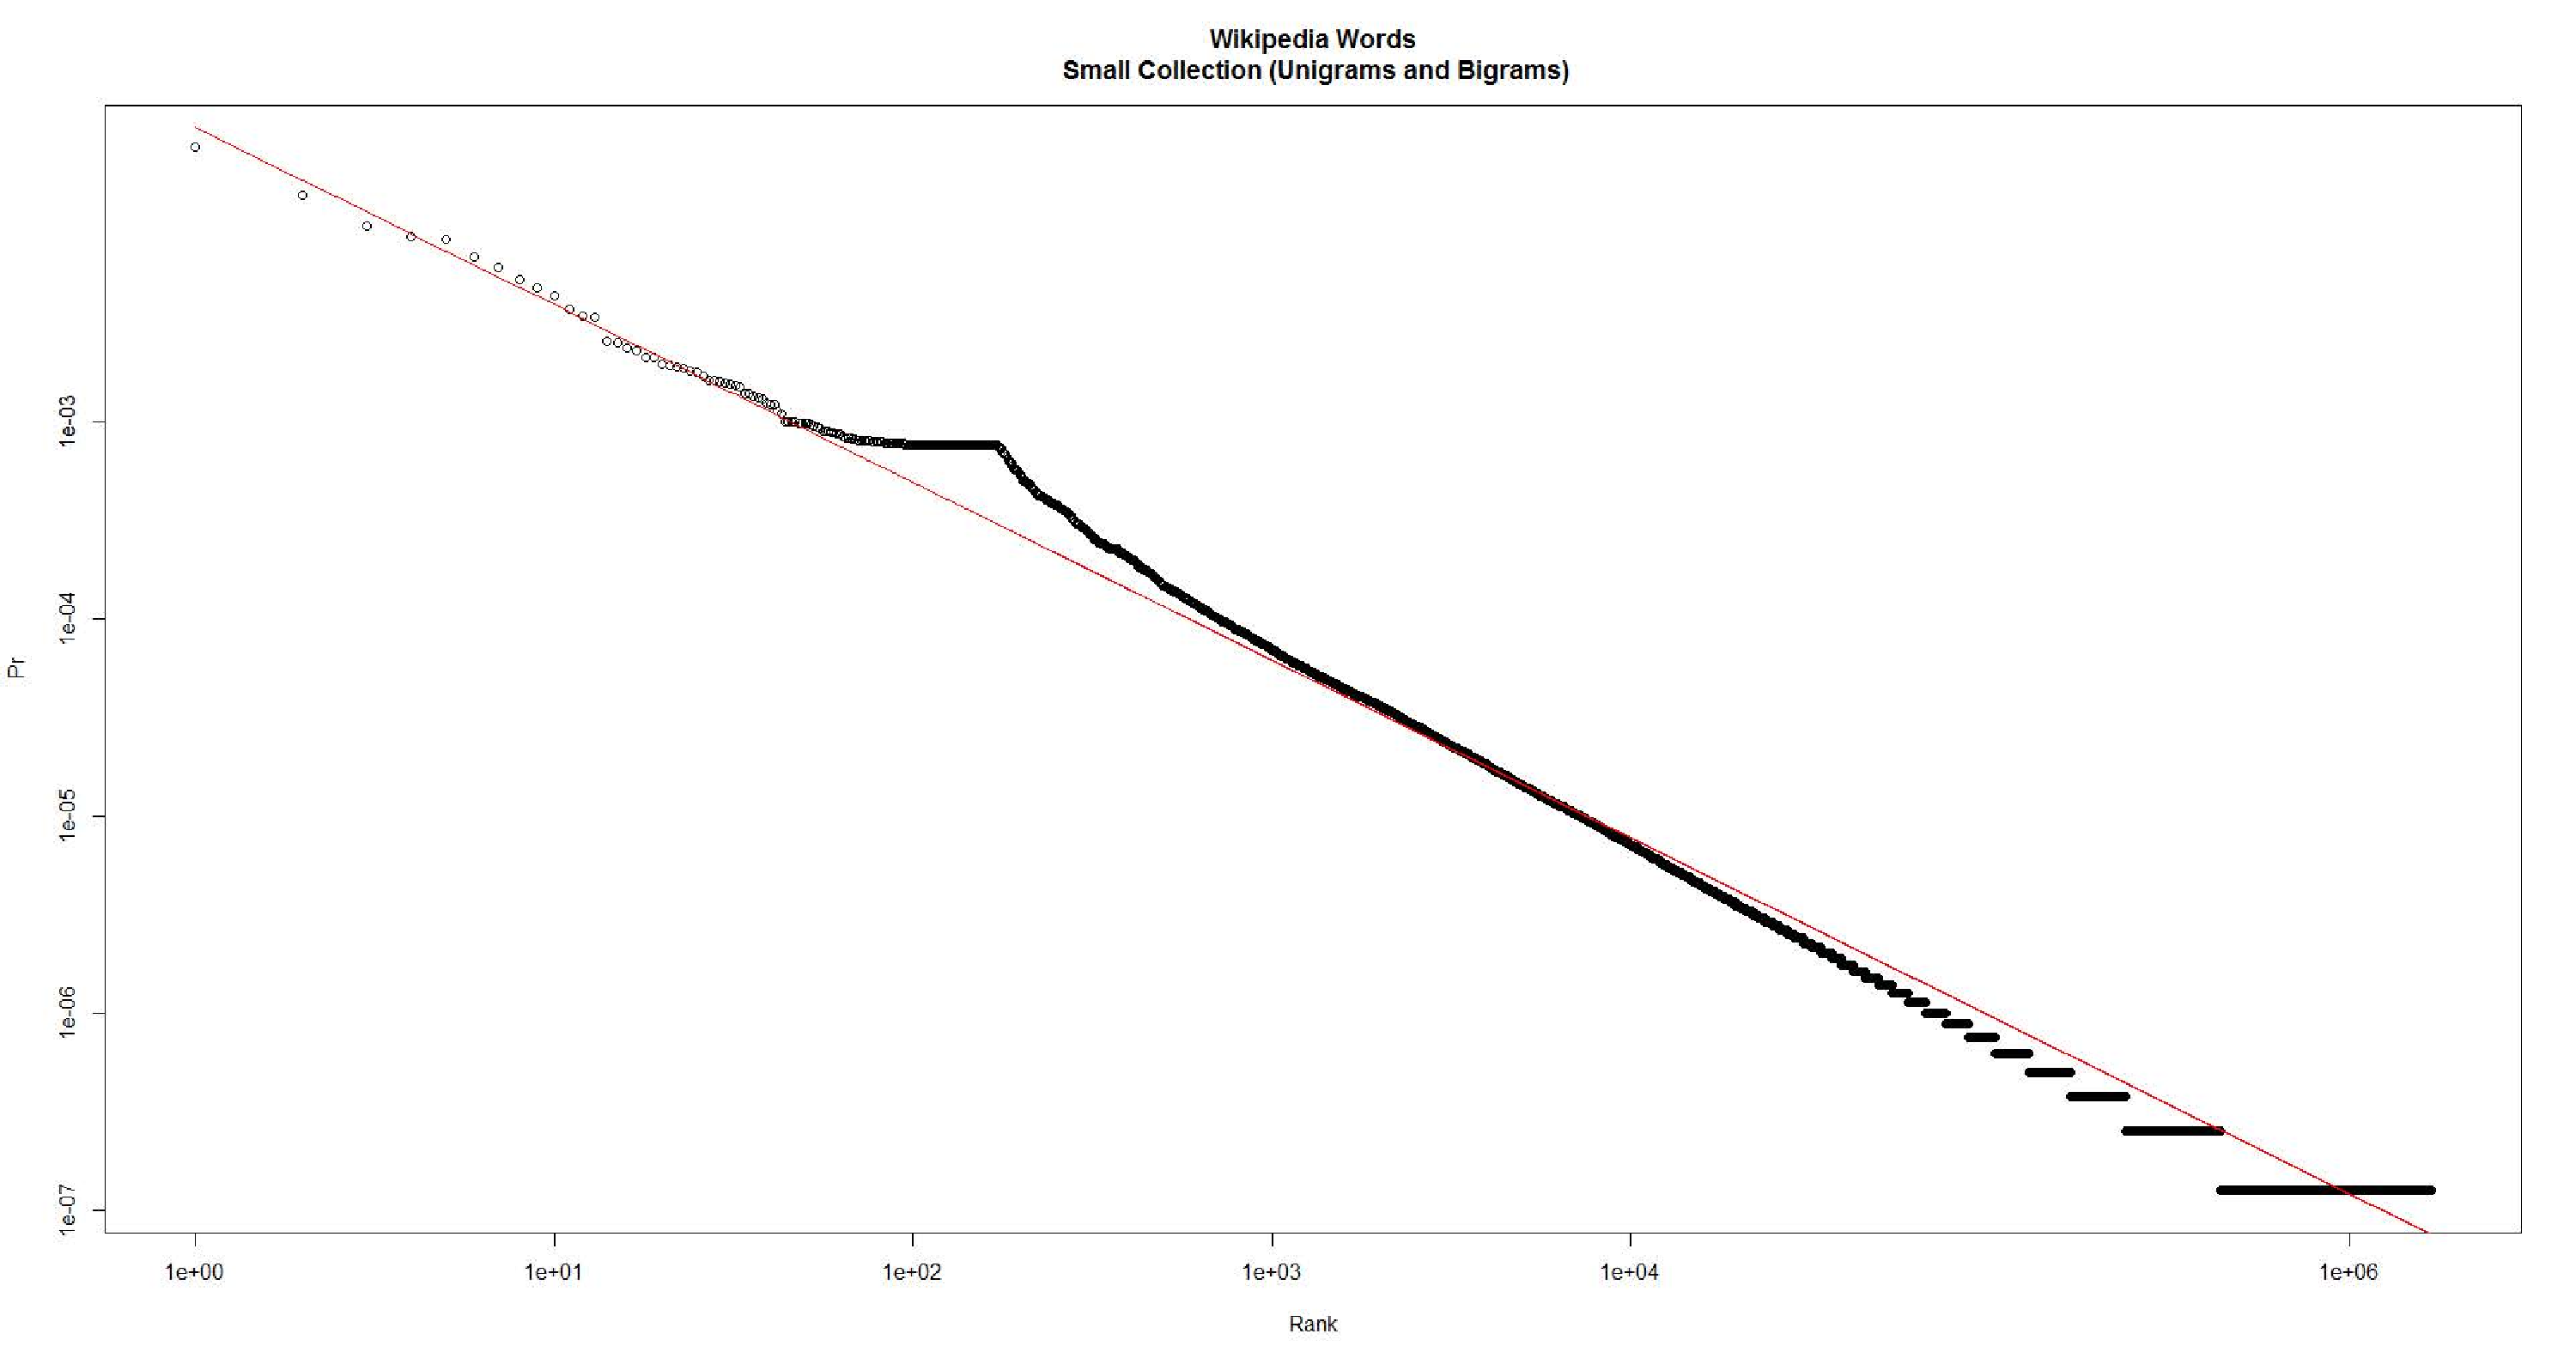
\includegraphics[scale=0.3]{images/zipf_cuve_s_combined.pdf}
\end{figure} 

\begin{verbatim}
Maximum likelihood estimation

Call:
mle(minuslogl = ll, start = list(s = 1))

Coefficients:
   Estimate   Std. Error
s 0.9232369 8.383762e-05

-2 log L: 178325957 
> exp(lzipf(s.sq,max_x))[1]
[1] 0.1117953
\end{verbatim}

Making $C$ for the combine curve = \textbf{0.1117953}
\end{homeworkProblem}
\newpage
%----------------------------------------------------------------------------------------
%	Problem 2
%----------------------------------------------------------------------------------------
\begin{homeworkProblem}[Exercise 4.2]% Custom section title
\vspace*{10pt} % Question 
Plot vocabulary growth for the Wikipedia collection and estimate the parameters
for Heaps’ law. Should the order in which the documents are processed
make any difference?\\
%--------------
%  P2 Approach
%--------------
\subsection{Approach}
Python script \textit{heaps\_curve.py}, shown on Listing \ref{listing:heaps-curve}, was developed to complete this exercise. The previous script \textbf{zipf\_curve.py} is very similar to \textit{heaps\_curve.py}. A modification was made to the previous solution to solve problem 2.\\

The main difference in this approach is that we tally the sum of all words in the dictionary as each document was processed, in line 71, ONLY \textit{unigram} tokens are used.
%--------------
%  zipf_curve.py
%--------------
\lstinputlisting[language=Python,
                 style=mybox, 
                 captionpos=t,
                 caption={heaps\_curve.py},
				 linerange={44-80},
				 firstnumber=44,                  
                 label=listing:heaps-curve,
                 ]
{../heaps_curve.py}

\subsubsection{Running Heaps\_curve.py}
\begin{figure}[h]\caption{Running Heaps\_curve.py from Command Line} \label{fig:run-heaps-curve}
	\center
	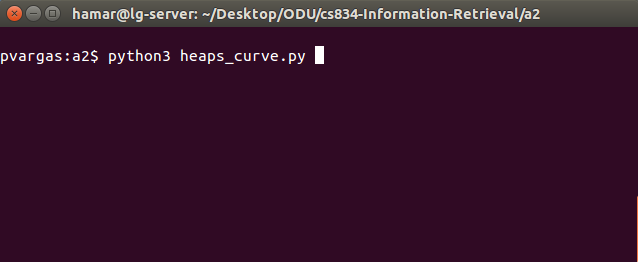
\includegraphics[scale=0.5]{images/run-heaps-curve.png}
\end{figure} 

%--------------
%  P2 SOlution
%--------------
\subsection{Solution}
\begin{figure}[h]\caption{Heaps-Curve for Wikepedia Small Collection} \label{fig:heaps-small}
	\center
	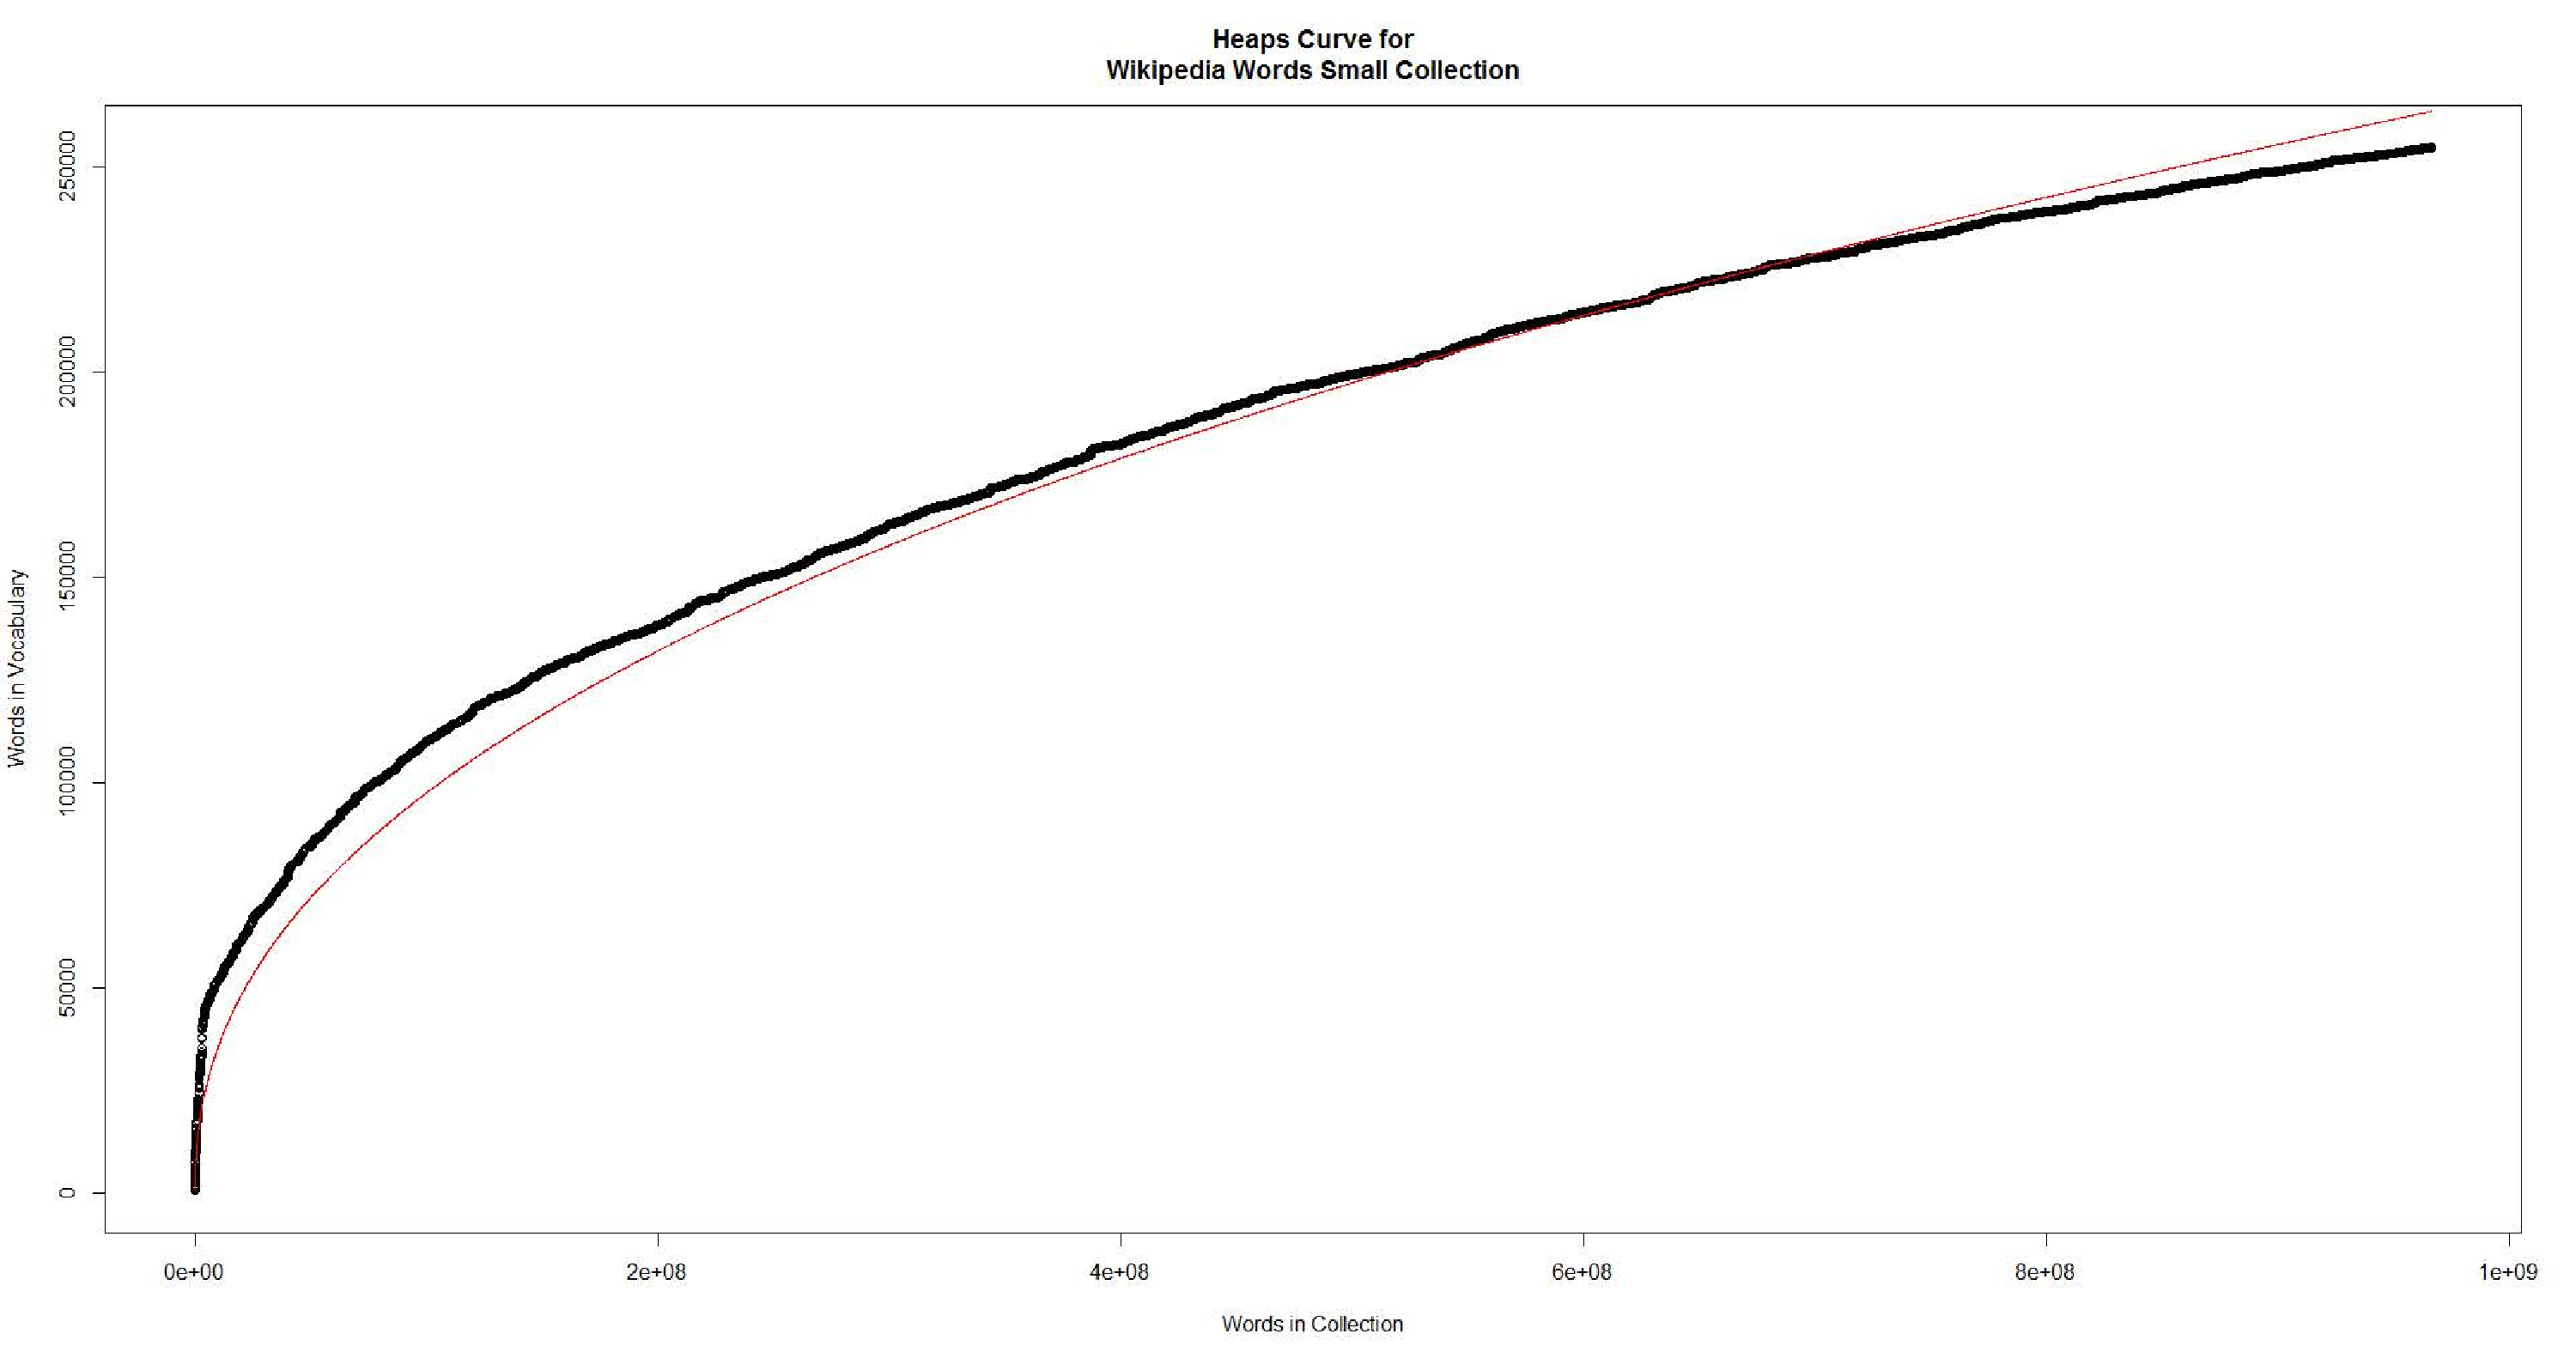
\includegraphics[scale=0.3]{images/heaps_cuve_s.pdf}
\end{figure} 

The red curve represents the prediction values for Wikipedia small collection  using function $v= K\dot{•}n^\beta$, where $K = 36$ and $\beta = 0.43$. The data for this curve is on the file \textit{heaps\_curve.txt}. It was plotted using the \textbf{R} script \textit{heaps\_curve.R}

\newpage
\begin{figure}[h]\caption{Heaps-Curve for Wikepedia Large Collection} \label{fig:heaps-large}
	\center
	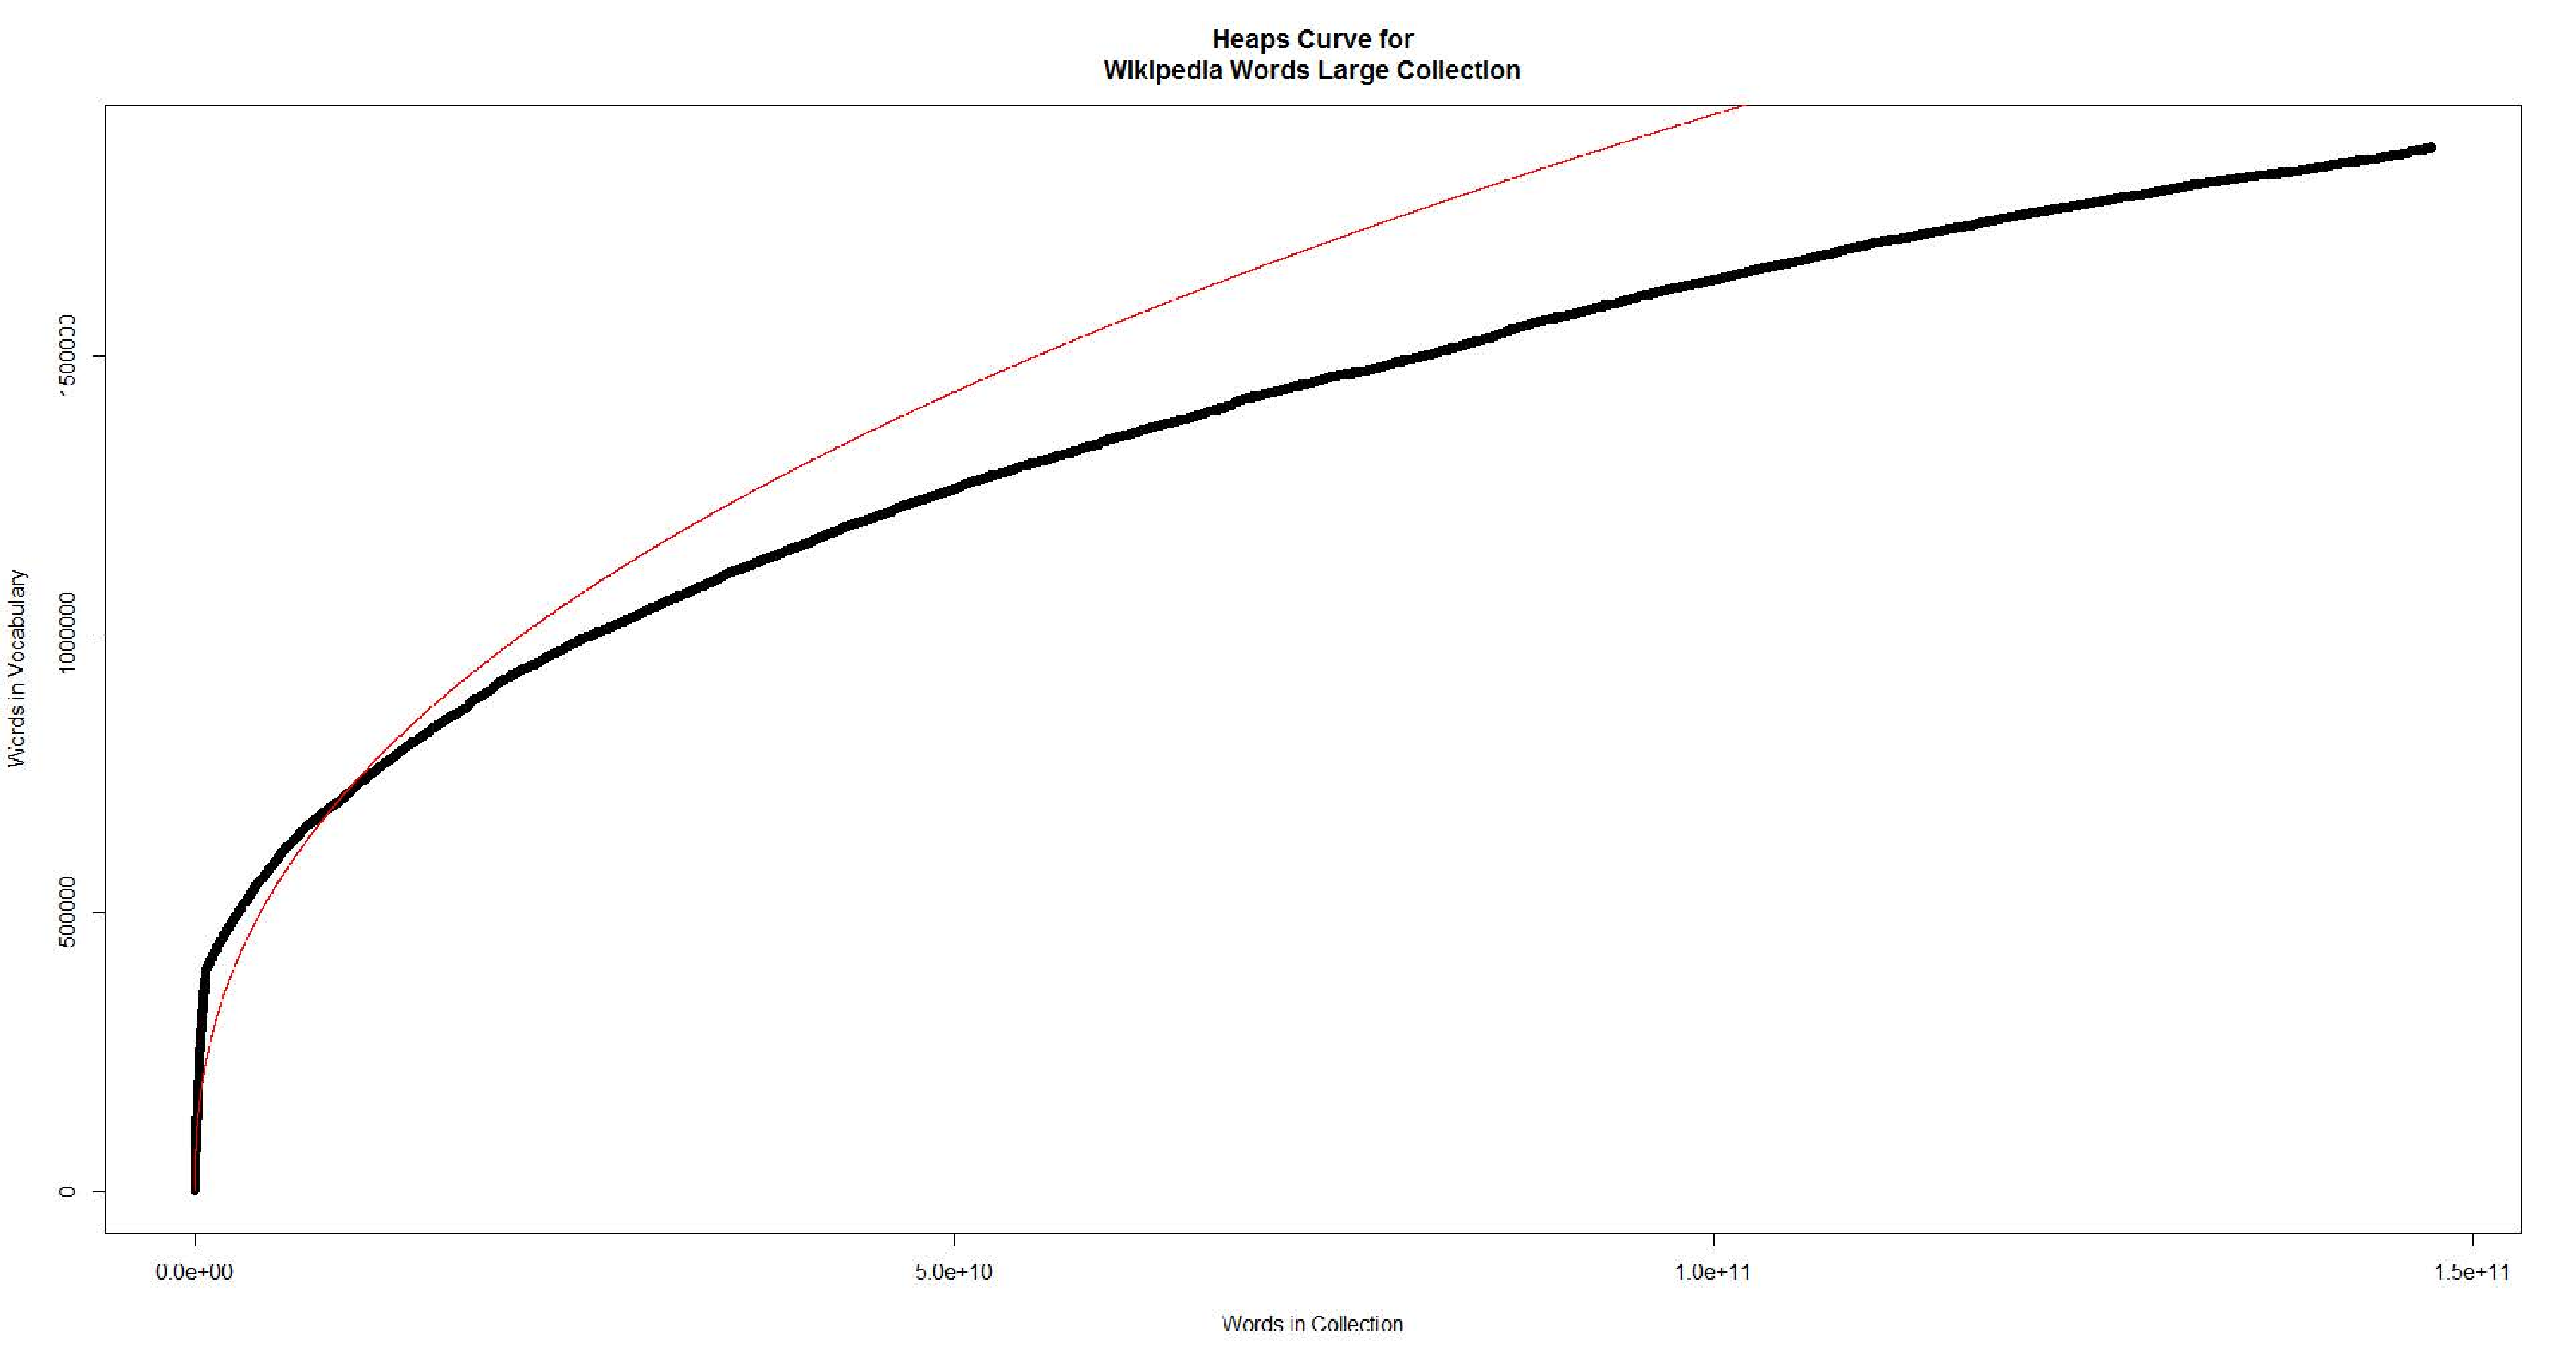
\includegraphics[scale=0.3]{images/heaps_cuve_l.pdf}
\end{figure} 

The red curve represents the prediction values for Wikipedia small collection for $v= K\dot{•}n^\beta$. The black curve was plotted using Wikipedia large collection values. Its data is contained in file \textit{heaps\_curve-l.txt}.

\end{homeworkProblem}
\newpage
%----------------------------------------------------------------------------------------
%	Problem 3
%----------------------------------------------------------------------------------------
\begin{homeworkProblem}[Exercise 4.3]% Custom section title
\vspace*{10pt} % Question 
Try to estimate the number of web pages indexed by two different search engines
using the technique described in this chapter. Compare the size estimates
from a range of queries and discuss the consistency (or lack of it) of these estimates.\\

\subsection{Approach}
According to the textbook \cite{CroftMetzlerStrohman} with the assumption that all terms occur independently:

\begin{equation}\label{eq:estimating-n}
  f_{ab} = N \cdot f_a/N \cdot f_b/N = (f_a \cdot f_b)/N
\end{equation}

Where:\\

$N$ is the number of documents in the collection.\\
$f_i$ is the number of document that term $i$ occurs.\\
$f_{ab}$ is the combined set result.\\

Then, we can estimate $N$ by:\\

\begin{equation}
	N = \frac{(f_a \cdot f_b)}{f_{ab}}
\end{equation}

\subsubsection{Search Engines}
The two search engines used for this exercise were: \textbf{Google} and \textbf{Bing}

\subsubsection{Query Terms}
The query term used for this experiment was: \textit{solar avocado}

\newpage
\subsection{Solution}
%--------------
%  P3 Google Estimation
%--------------
\subsubsection{Google Estimation}
Looking at Figure \ref{fig:google-solar}:
\begin{equation*}
	f_{solar} = 623,000,000
\end{equation*}
Looking at Figure \ref{fig:google-avocado}:
\begin{equation*}
	f_{avocado} = 70,700,000
\end{equation*}

Looking at Figure \ref{fig:google-solar-avocado}:
\begin{equation*}
	f_{solar\ avocado} = 562,000
\end{equation*}

\newpage
\begin{figure}[h]\caption{Google Solar Term} \label{fig:google-solar}
	\center
	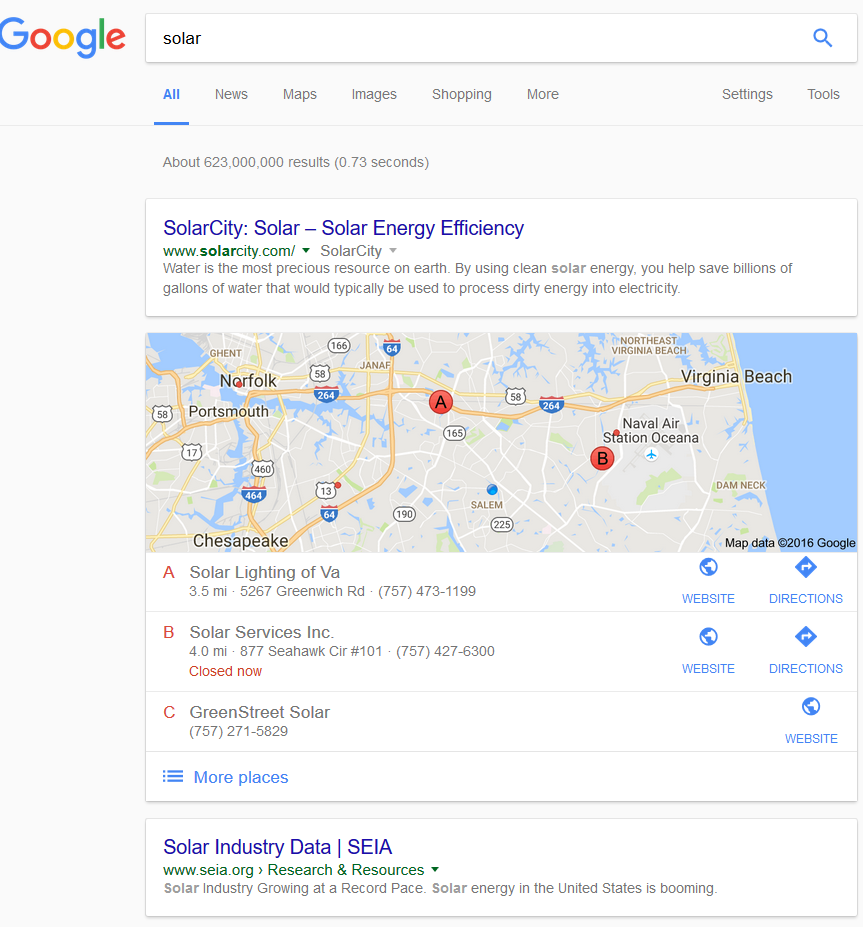
\includegraphics[scale=0.5]{images/google_solar.png}
\end{figure} 
\newpage
\begin{figure}[h]\caption{Google Avocado Term} \label{fig:google-avocado}
	\center
	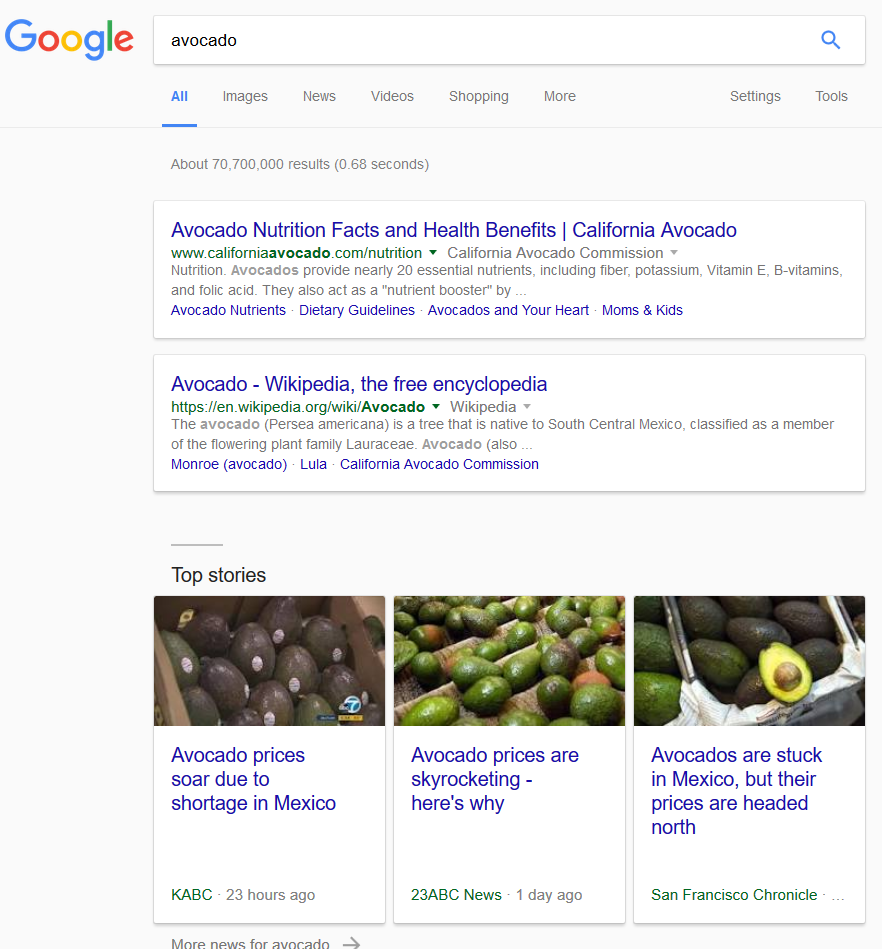
\includegraphics[scale=0.5]{images/google_avocado.png}
\end{figure}

\newpage
\begin{figure}[h]\caption{Google Solar Avocado Term} \label{fig:google-solar-avocado}
	\center
	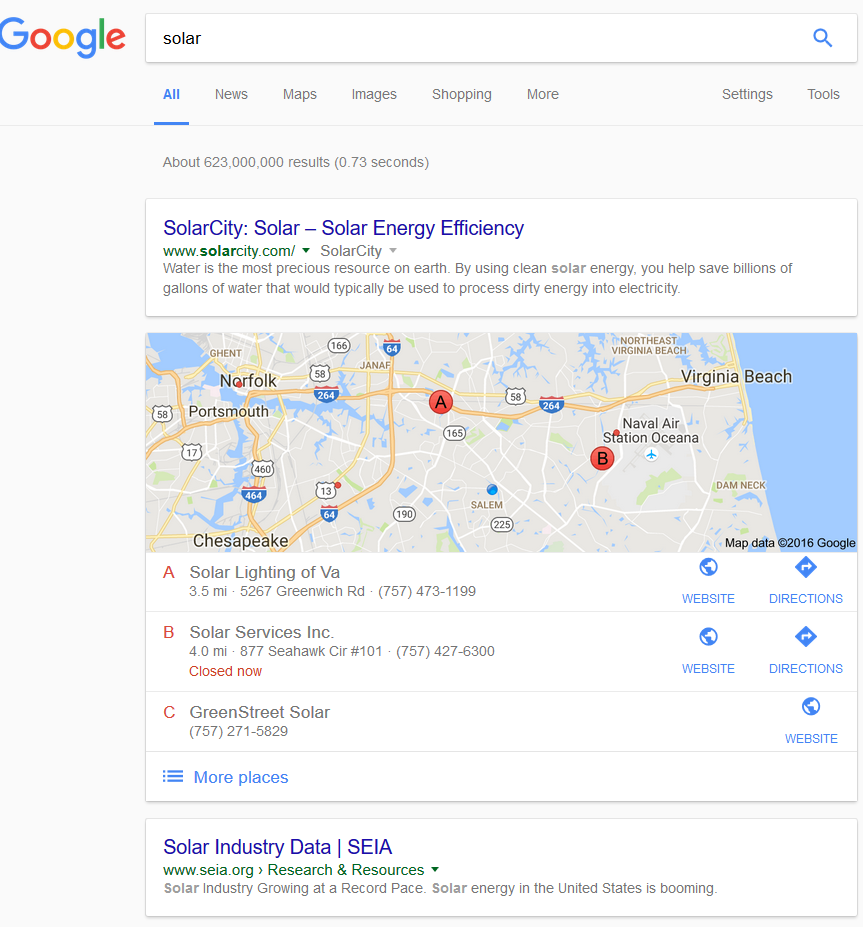
\includegraphics[scale=0.5]{images/google_solar.png}
\end{figure}

\newpage
\paragraph{Google Estimation of $N$}
From equation (\ref{eq:estimating-n}) we can estimate the value of $N$ by:
\begin{equation*}
	N = \frac{(623,000,000 \cdot 70,700,000)}{562,000}
\end{equation*}
\begin{equation*}
	N = 78.4\ billion
\end{equation*}

\vspace{5mm}
Making a comparison with Figure \ref{fig:google-size}, our estimation is 78.4/45.5 or approximately three quarters larger of the size estimated in \url{http://www.worldwidewebsize.com/}. \\

\begin{figure}[h]\caption{Google Collection Size} \label{fig:google-size}
	\center
	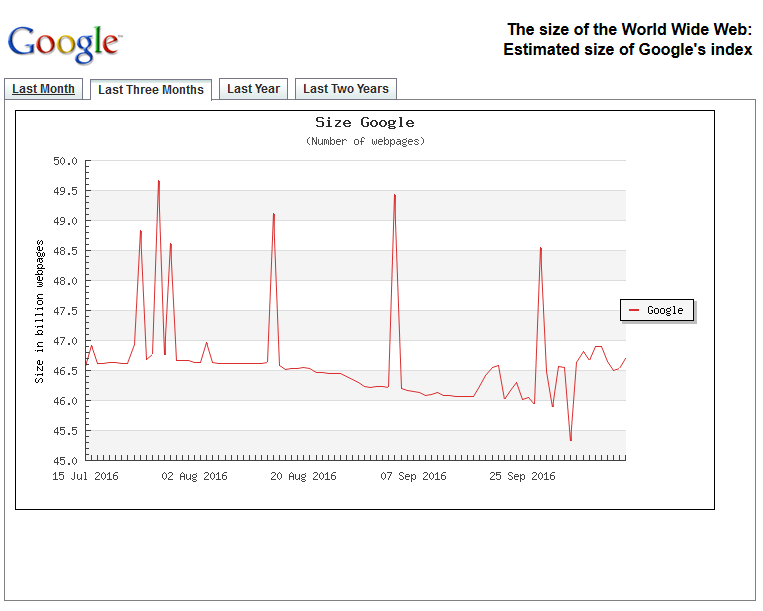
\includegraphics[scale=0.5]{images/google_size.png}
\end{figure}
%--------------
%  P3 Bing Estimation
%--------------
\newpage
\subsubsection{Bing Estimation}
Looking at Figure \ref{fig:bing-solar}:
\begin{equation*}
	f_{solar} = 44,900,000
\end{equation*}
Looking at Figure \ref{fig:bing-avocado}:
\begin{equation*}
	f_{avocado} = 13,900,000
\end{equation*}

Looking at Figure \ref{fig:bing-solar-avocado}:
\begin{equation*}
	f_{solar\ avocado} = 811,000
\end{equation*}
\begin{figure}[h]\caption{Bing Solar Term} \label{fig:bing-solar}
	\center
	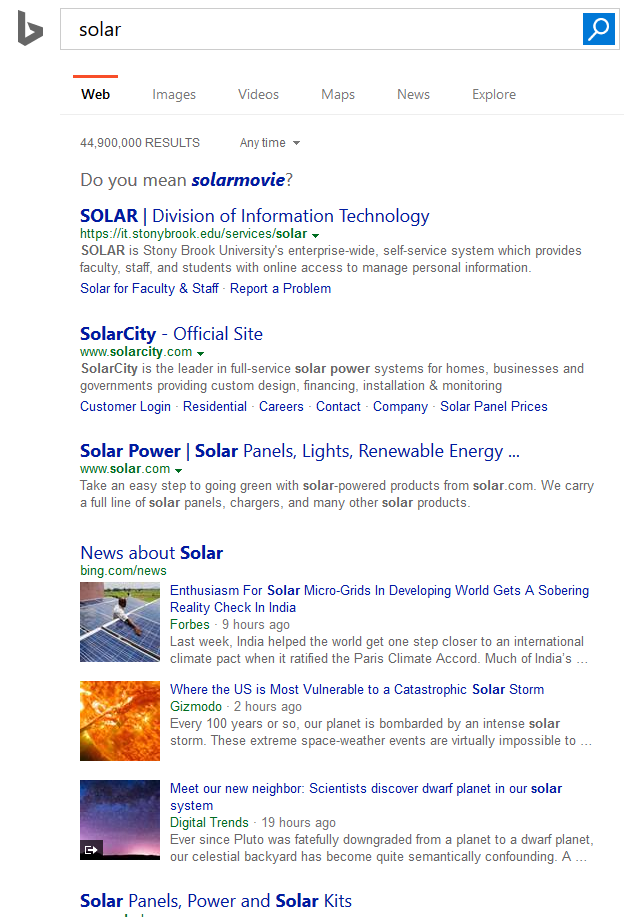
\includegraphics[scale=0.5]{images/bing_solar.png}
\end{figure} 
\newpage
\begin{figure}[h]\caption{Bing Avocado Term} \label{fig:bing-avocado}
	\center
	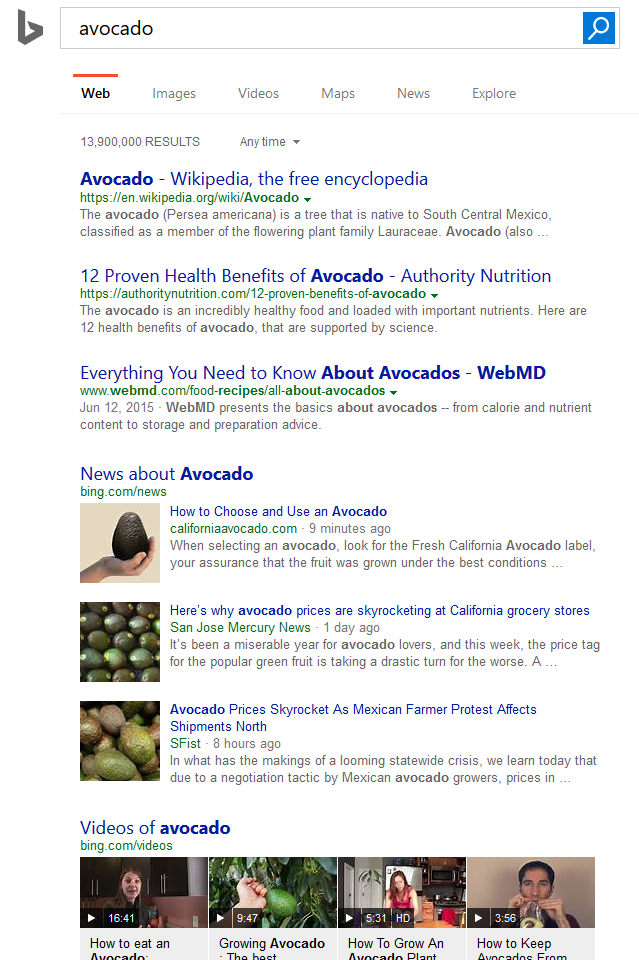
\includegraphics[scale=0.5]{images/bing_avocado.png}
\end{figure}
\newpage
\begin{figure}[h]\caption{Bing Solar Avocado Term} \label{fig:bing-solar-avocado}
	\center
	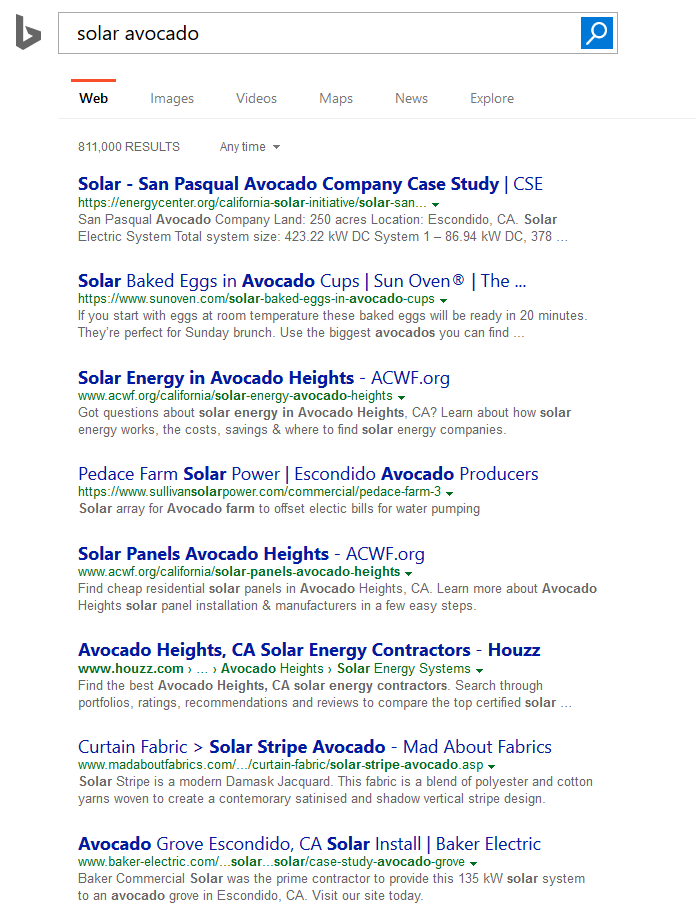
\includegraphics[scale=0.5]{images/bing_solar_avocado.png}
\end{figure}

% ------------------------------
%  Bing Estimation
% ------------------------------
\newpage
\paragraph{Bing Estimation of $N$}
From equation (\ref{eq:estimating-n}) we can estimate the value of $N$ by:
\begin{equation*}
	N = \frac{(44,900,000 \cdot 13,900,000)}{811,000}
\end{equation*}
\begin{equation*}
	N = 77\ million
\end{equation*}

Making a comparison with Figure \ref{fig:bing-size}, our estimation is 77/1600 or approximately 5 percent of the size estimated in \url{http://www.worldwidewebsize.com/}. 

\begin{figure}[h]\caption{Bing Collection Size} \label{fig:bing-size}
	\center
	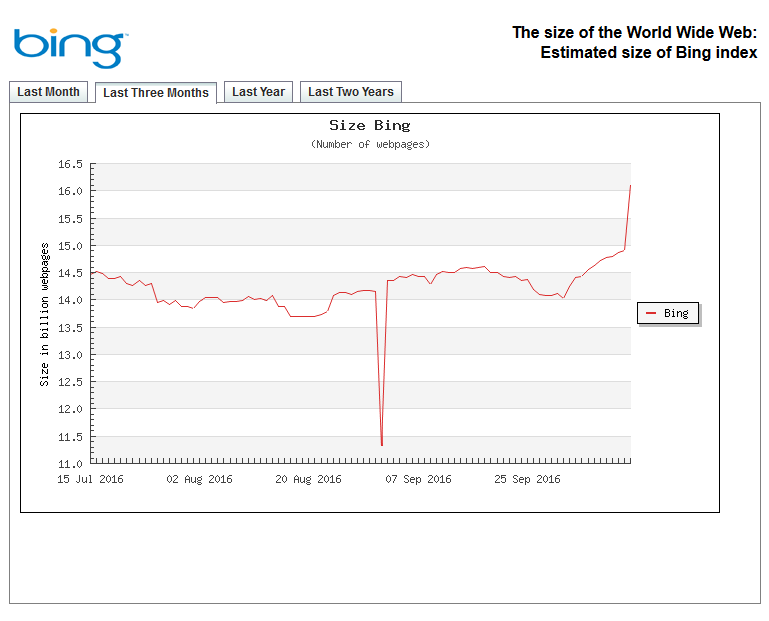
\includegraphics[scale=0.5]{images/bing_size.png}
\end{figure}

\newpage
\end{homeworkProblem}
%----------------------------------------------------------------------------------------
%	Problem 4
%----------------------------------------------------------------------------------------
\begin{homeworkProblem}[Exercise 4.8]% Custom section title
Find the 10 Wikipedia documents with the most inlinks. Show the collection
of anchor text for those pages
\vspace*{10pt} % Question 

%--------------
%  P4 Approach
%--------------
\subsection{Approach}
The task was divided into two sub-problems: \textbf{counting links} and \textbf{pairing links} with actual resources. The python script \textit{inklinks.py} (see Listing \ref{listing:inlinks}) was developed to solve this problem. There were many links pointing to relative non-existent links within the collection. 

\subsubsection{Running Inlinks.py}
\begin{figure}[h]\caption{Running Inlinks.py} \label{fig:run-inlinks}
	\center
	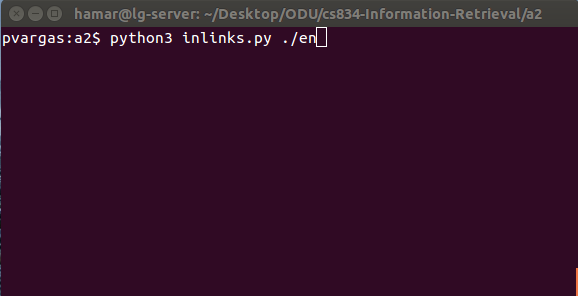
\includegraphics[scale=0.5]{images/run-inlinks.png}
\end{figure} 

\subsubsection{Counting Links}
Two dictionaries are created: \textbf{crawled\_pages} and \textbf{link\_count}. The first keeps track of all resources retrieved from the collection. Its key is the URI of the collection. Its value is initialized to zero (line 24). All the links in the HTML page are extracted and added to second dictionary. See lines 37-45 in Listing \ref{listing:inlinks}.

\begin{figure}[h]\caption{Inlinks Dictionary} \label{fig:inlinks-dict}
	\center
	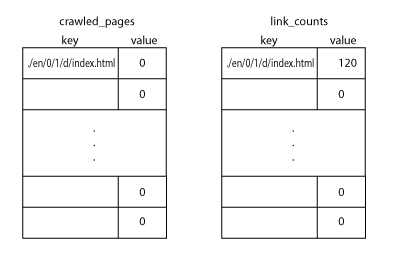
\includegraphics[scale=0.5]{images/inlinks.png}
\end{figure} 

\subsubsection{Pairing Links}
Finally, the crawled pages are looked in the link counts. The value for similar keys is transferred to the \textbf{crawled\_pages} dictionary (see lines 56-58 in Listing \ref{listing:inlinks}). This will guarantee that only valid resources will be considered for inlinks counts. The dictionary is sorted in descend order (line 61) and the top-10 inlinks are saved into file \textit{anchor-text.txt} with their anchor texts. See lines 77-84. 
%--------------
%  inlinks.py
%--------------
\lstinputlisting[language=Python,
                 style=mybox, 
                 captionpos=t,
                 caption={inlinks.py},
				 linerange={21-90},
				 firstnumber=21,                  
                 label=listing:inlinks,
                 ]
{../inlinks.py} 
\subsection{Solution}
The solution is the file \textbf{anchor-text.txt} uploaded under a2 folder in github.
\end{homeworkProblem}
%----------------------------------------------------------------------------------------
%	Problem 5
%----------------------------------------------------------------------------------------
\begin{homeworkProblem}[Exercise 5.10]% Custom section title
\vspace*{10pt} % Question 
5.10. Suppose a company develops a new unambiguous lossless compression
scheme for 2-bit numbers called SuperShrink. Its developers claim that it will reduce
the size of any sequence of 2-bit numbers by at least 1 bit. Prove that the
developers are lying. More specifically, prove that either:
\begin{itemize}
\item SuperShrink never uses less space than an uncompressed encoding, or
\item There is an input to SuperShrink such that the compressed version is larger than the uncompressed input
\end{itemize}
You can assume that each 2-bit in put number is encoded separately.

\subsection{Solution}
The \textit{SuperShrink} encryption will have to encode the following 2-bits numbers:
\[ 
\left \{
  \begin{tabular}{c}
  00\\
  01\\
  10\\ 
  11
  \end{tabular}
\right \}
\]

The smallest sequence will have $2^4$ possible scenarios:

\begin{center}
\begin{tabular}{r|l}
00&00\\
00&01\\
00&10\\
00&11\\
01&00\\
01&01\\
01&10\\
01&11\\
10&00\\
10&01\\
10&10\\
10&11\\
11&00\\
11&01\\
11&10\\
11&11\\
\end{tabular} 
\end{center}
We will need $Log_2(2^4)$ bits or 4 bits to account for each outcome in an unambiguous scheme. If we remove one bit to encode 4-bit sequence, what would be the decoding of sequence 111? it could be 1111 or 0111 if we truncate the head. It could be 1111 or 1110 if we truncate the tail. 

\end{homeworkProblem}
%----------------------------------------------------------------------------------------
%	Bibliography
%----------------------------------------------------------------------------------------
\newpage
\bibliography{bibliography}
\bibliographystyle{siam}
%\begin{thebibliography}{9}
%\bibitem{Lutz} 
%Lutz, Mark (2013). List and Dictionaries. \textit{Learning Python} (5th ed.). (pp. %262-263). Sebastopol, CA: O'Reilly Media.
%
%\bibitem{ci}
%Segarn, Toby. Programming Collective Intelligence. \textit{Building Smart Web 2.0 Application}. (pp 29-53). Sebastopol, CA: O'Reilly Media.

%\bibitem{sitemaps}
%Sitemaps Schema. (n.d.) Retrieved September 21, 2016, from \url{http://www.sitemaps.org/schemas/sitemap/0.9}

%\end{thebibliography}
\end{document}

